The SiPMs were used in the TRITIUM experiment in two different ways, at the level of a single SiPM and at the level of several SiPMs arranged in a matrix. Both studies were carried out to learn about the detection with them and to characterize the SiPM arrays used in the TRITIUM monitor.

The electronic system used to process and analyze the output signals of the SiPM arrays is PETSYS \cite{PETSYS}, which is a commercial system prepared to work with SiPM matrices from Hamamatsu.

Petsys system, Figure \ref{fig:PETSYS}, is a complete acquisition and digitization system that is capable of working with up to 1024 SiPM. It consists of a basic board, which processes the signal, to which 8 different SiPM matrices can be connected with up to 64 SiPM per matrix. This number of channels is needed in the TRITIUM project because, as it is shown in section \ref{sec:TritiumMonitor}, the TRITIUM monitor use dozens of SiPM matrices with 16 channels (SiPMs) per matrix.

\begin{figure}[htbp]
\centering
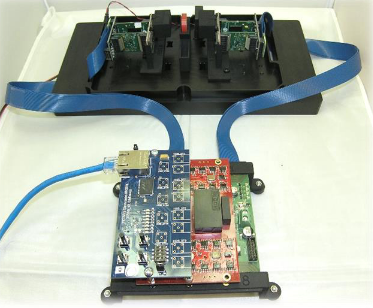
\includegraphics[scale=0.6]{3DesignPrinciples/32Tritium_detector/PETSYS_System.png}
\caption{Different parts of PETSYS system.\label{fig:PETSYS}~\cite{PETSYS}}
\end{figure}

Although the capacity provided by PETSYS should be enough for the requirements of the TRITIUM project, TRITIUM is a modular detector with scalable sensitivity. It means that, if an inprovement of its achieved limits is needed (improve its sensitivity or further reduce the background) more photosensors are needed. Therefore, the electronic system used should be able to increase its capacity in a scalable way. This requisit is fulfilled by PETSYS since it has an additional module, called Clock and Trigger, with which up to sixteen different PETSYS basic boards can be connected. Theses sixteen Petsys basic boards are read in parallel, each with the capacity previously mentioned, giving a total system capacity of 256 SiPM matrices (16384 SiPMs\footnote{$1024\cdot{}16 = 16384$}).

PETSYS is based on C++ and Python scripts that are prepared for the main tasks required for our experiment, such as time coincidence options between SiPM (or even SiPM matrices) or energy discrimination. It is open source, giving the possibility to modify the current scripts or develop others with additional functions. %The way the signals will be processed and analyzed for PETSYS will be exactly the same as those shown in Figure \ref{fig:ElectronicConfiguraitonsPMT}

This system has a time resolution of $250~\pico\second$ which is one of the best time resolutions of commercial systems available today and its price is around $10$\euro$/$ channel, which is a cheaper price compared to current similar electronic systems.

As we will see in section \ref{sec:CharacterizationSiPM}, the temperature of each SiPM matrix is an important parameter to take into account. The PETSYS system has the ability to monitor the temperature of both, the SiPM matrices and ASICS that are used to control them during the measurements. It is an important parameter to ensure the correct functioning of both, the photosensors and the system, and it offers the possibility of developing new function scripts that allow to implement the stability gain method shown in section \ref{sec:CharacterizationSiPM}.

Although TRITIUM monitor use SiPM matrices it is important to start the characterizaton at the level of a single channel (only one SiPM) since its reduce the uncertainties in the first results.

%Although PETSYS is the system used to work with SiPM matrices in the TRITIUM detector, it does not allow characterizing the SiPMs, which is an important task to understand the results of our detector.

In order to do so, an electronic system was designed, developed and built with which we can read up to eight different SiPMs and it has the capacity to monitor the temperature.

This system is based on three different PCBs\footnote{PCB, Printed Circuit Board}, shown in Figure \ref{fig:PCBs_LEDSpectrum} and whose electronical schemes are shown in the appendix \ref{App:ElectronicalSchemesSiPMPCBs}, the output signal of which is connected to an oscilloscope to process and analyze the signal:

\begin{enumerate}
\item{} The first PCB, shown in Figure \ref{subfig:PCB1}, is used to organize the SiPMs and sensor temperature in this system. This PCB place up to 8 different SiPMs and a temperature sensor and arrange their output signals on two HDMI connections.

This PCB is placed inside a special black box, from "" company, that has a high degree of light tightness. This black box has a small hole, whose diameter is $1~\mm$, prepared to introduce an optical fiber\footnote{The optical fiber used is BCF-98 from Saint-Gobain company \cite{OpticalFibers}} with which the SiPM can be iluminated with a incoherent light source. The light source used is a LED, model 430L from Thorlabs company \cite{LEDThorlabs}, whose emission spectrum is shown in Figure \ref{subfig:LEDSpectrum}, which has been experimentaly measured using a spectrometer and fitted to a Gaussian function. We can see that the emission peak of this LED is produced at $436.3$ with a FWHM\footnote{The FWHM parameter, Full Width at Half Maximum, of a Gaussian fit can be calculated from its sigma using the equation: FWHM$=2.35 \cdot{} \sigma$} of $19.1~\nano\meter$. With this LED we intend to simulate the light emission of the fibers used in the TRITIUM experiment to calibrate the SiPMs at the working wavelength. 

\item{} The second PCB, shown in Figure \ref{subfig:PCB2}, is used to sum the different signals of the SiPMs and amplify them by a factor $G=4187.5$ or $G=10761.88$ depends on the input resistance oscilloscope, $50~\varOmega$ or $1~\mega\varOmega$, respectively. This PCB uses a differential amplification with which the electronic noise of the system is reduced and it is connected to the first PCB through two HDMI feedthroughs.

\item{} The third PCB, shown in Figure \ref{subfig:PCB3}, is used to arrange all the different input and output signals of this system in an HDMI connection without introducing electrical noise by crosstalk between different signals. This PCB is connected to the second PCB trought a HDMI feedthrough.

The input signals of this system are the supply voltage of the SiPMs and the supply voltage of the PCBs ($\pm 6~\volt$) and the output signals are the temperature sensor signal and the summed signal of all SiPMs. 

\end{enumerate}

\begin{figure}[htbp]
 \centering
  \subfloat[PCB 1 used to arrang 8 SiPMs and black box.]{
   \label{subfig:PCB1}
    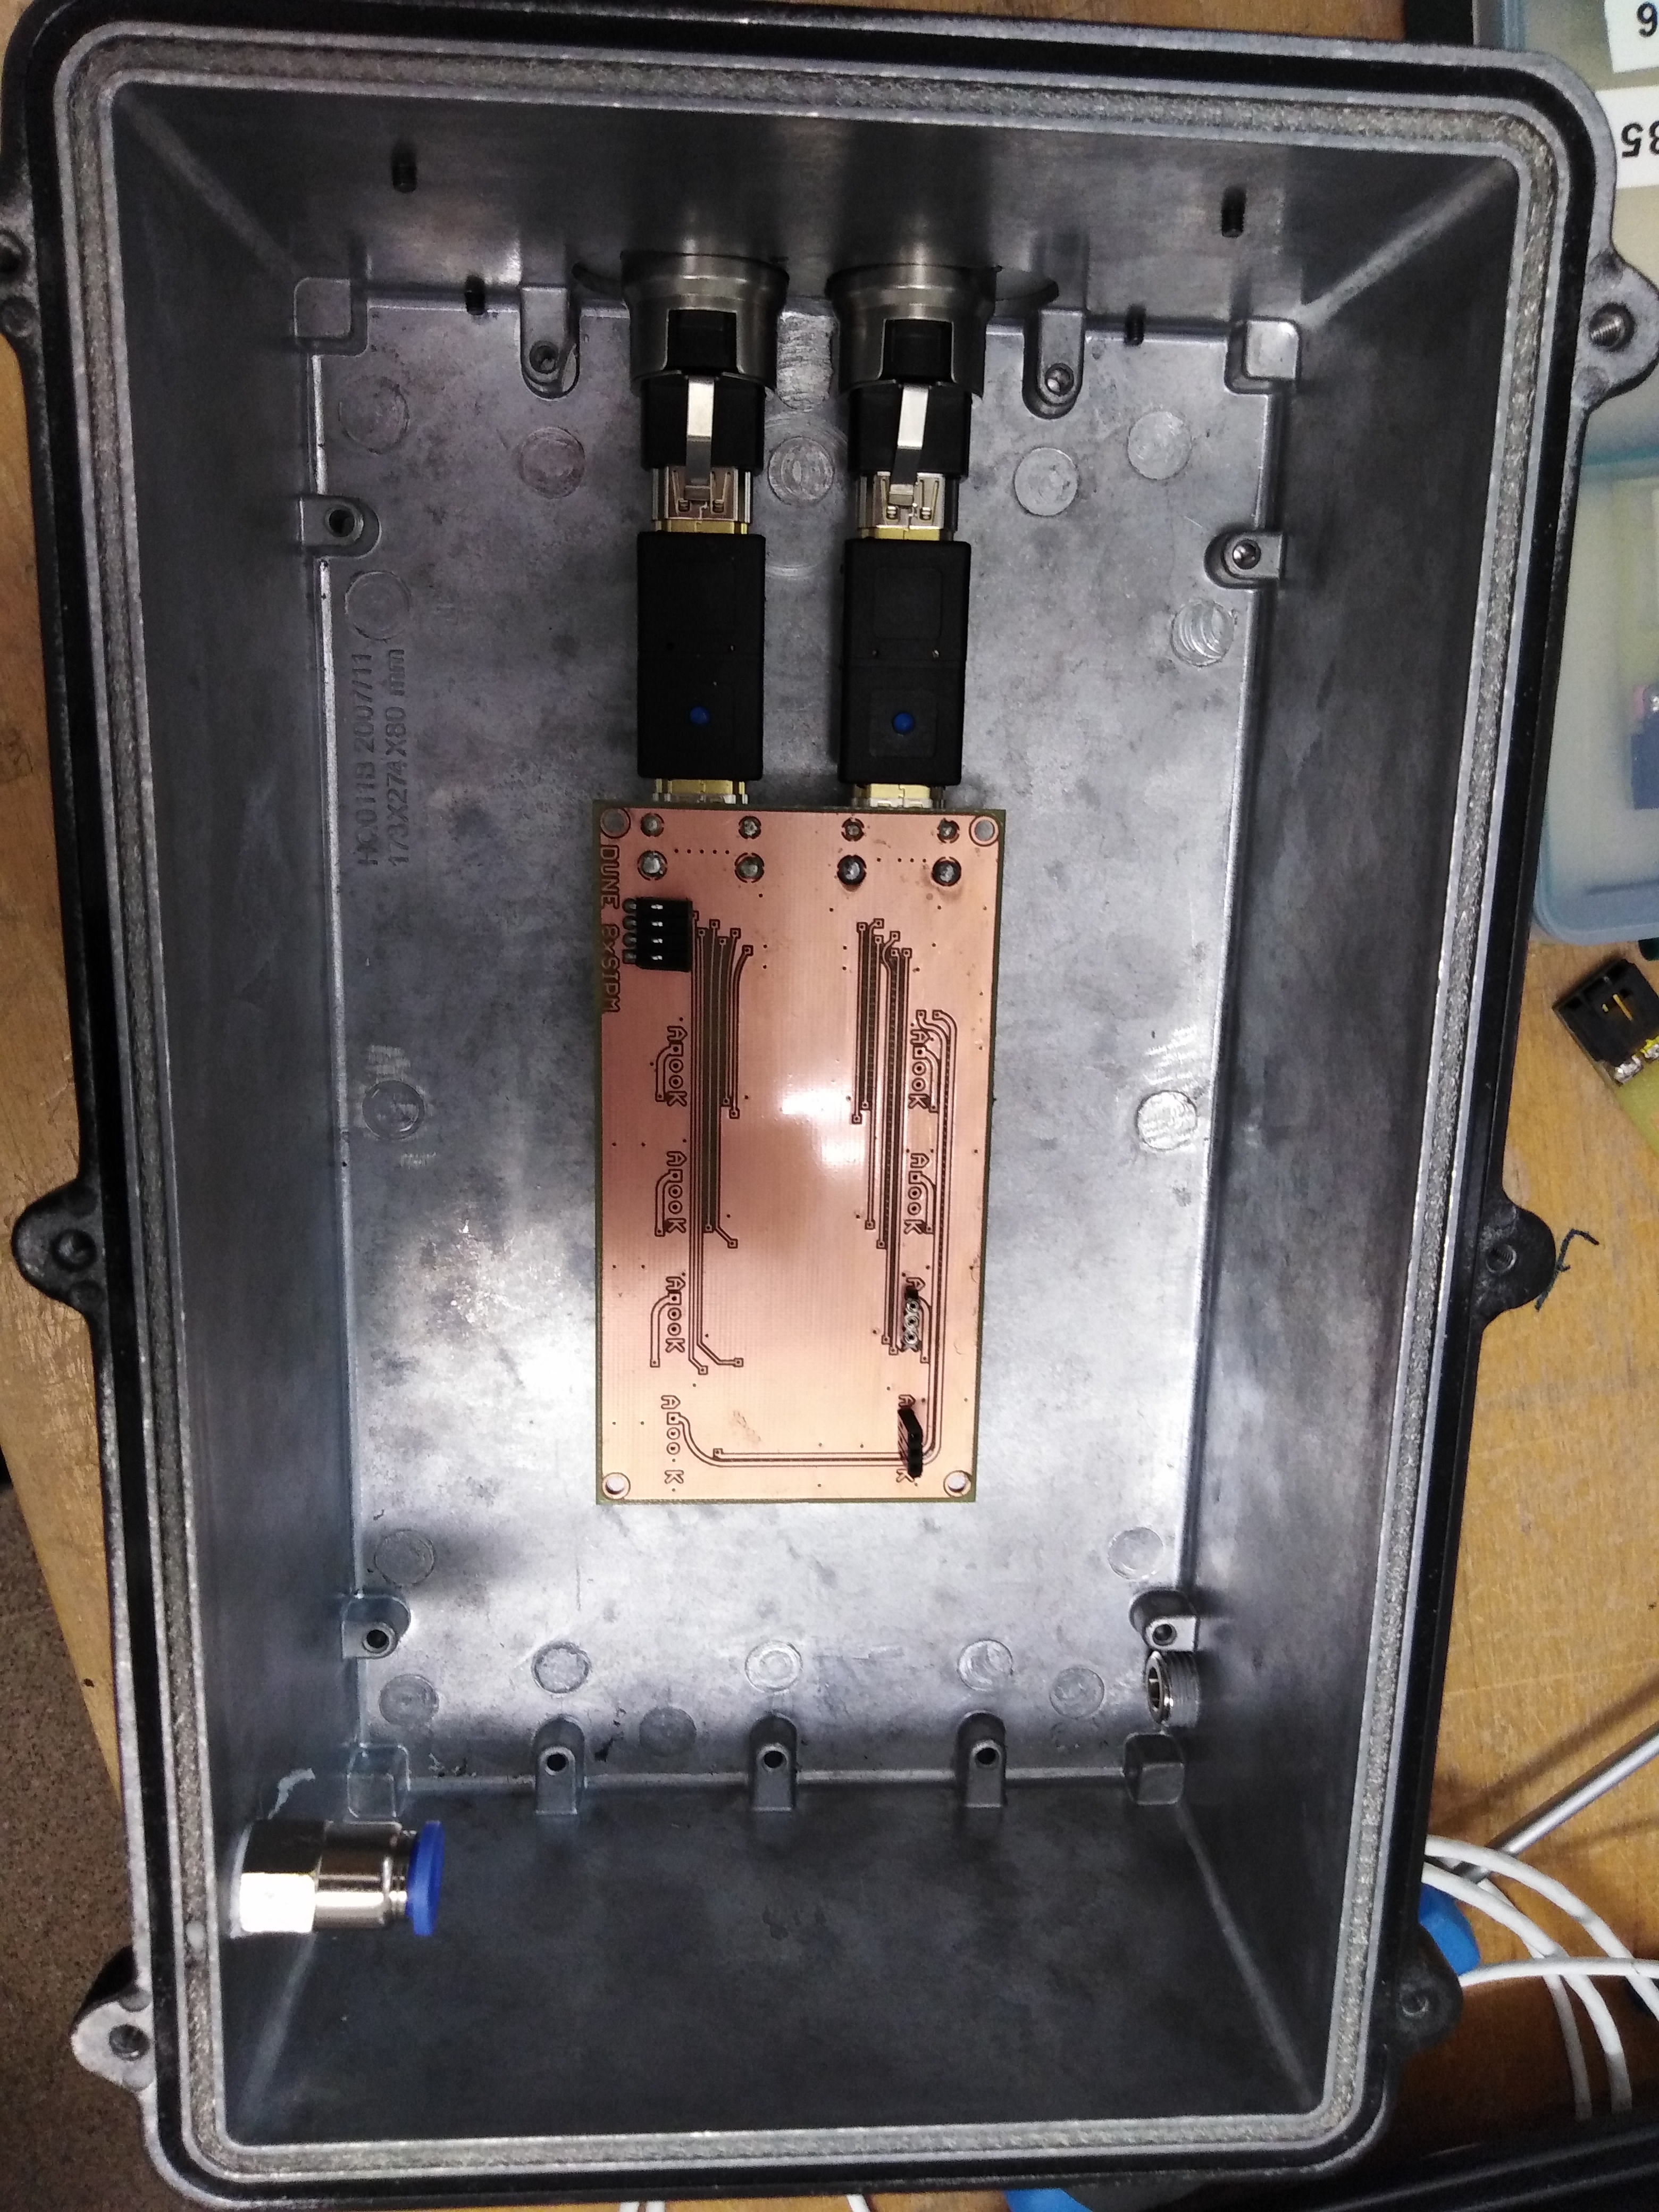
\includegraphics[angle=90,width=0.5\textwidth]{3DesignPrinciples/32Tritium_detector/PCB1_SiPM_Black_Box.jpg}}
  \subfloat[PCB 2 used to sum and amplify the output signals of SiPMs]{
   \label{subfig:PCB2}
    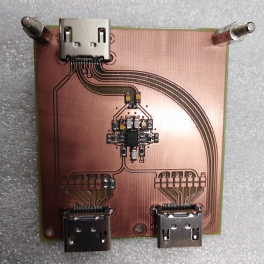
\includegraphics[width=0.45\textwidth]{3DesignPrinciples/32Tritium_detector/PCB2_SIPMs.png}}
   \newline
  \subfloat[PCB 3 used to arrange the different singals of the system.]{
   \label{subfig:PCB3}
    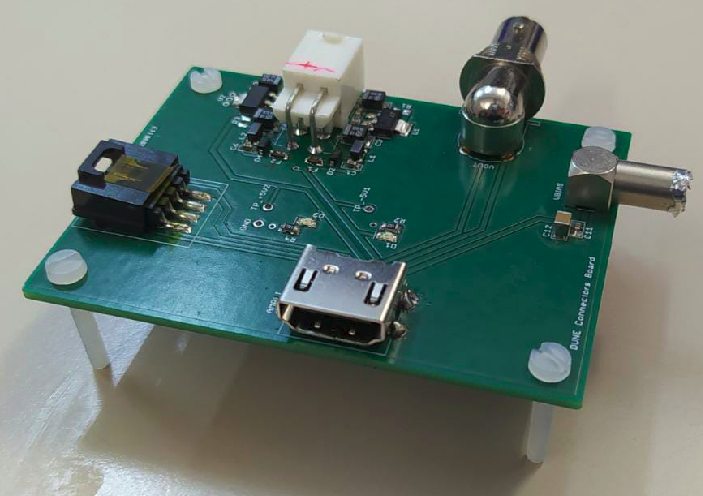
\includegraphics[width=0.4\textwidth]{3DesignPrinciples/32Tritium_detector/PCB3_SiPMs.png}}
  \subfloat[Emission spectrum of the LED.]{
   \label{subfig:LEDSpectrum}
    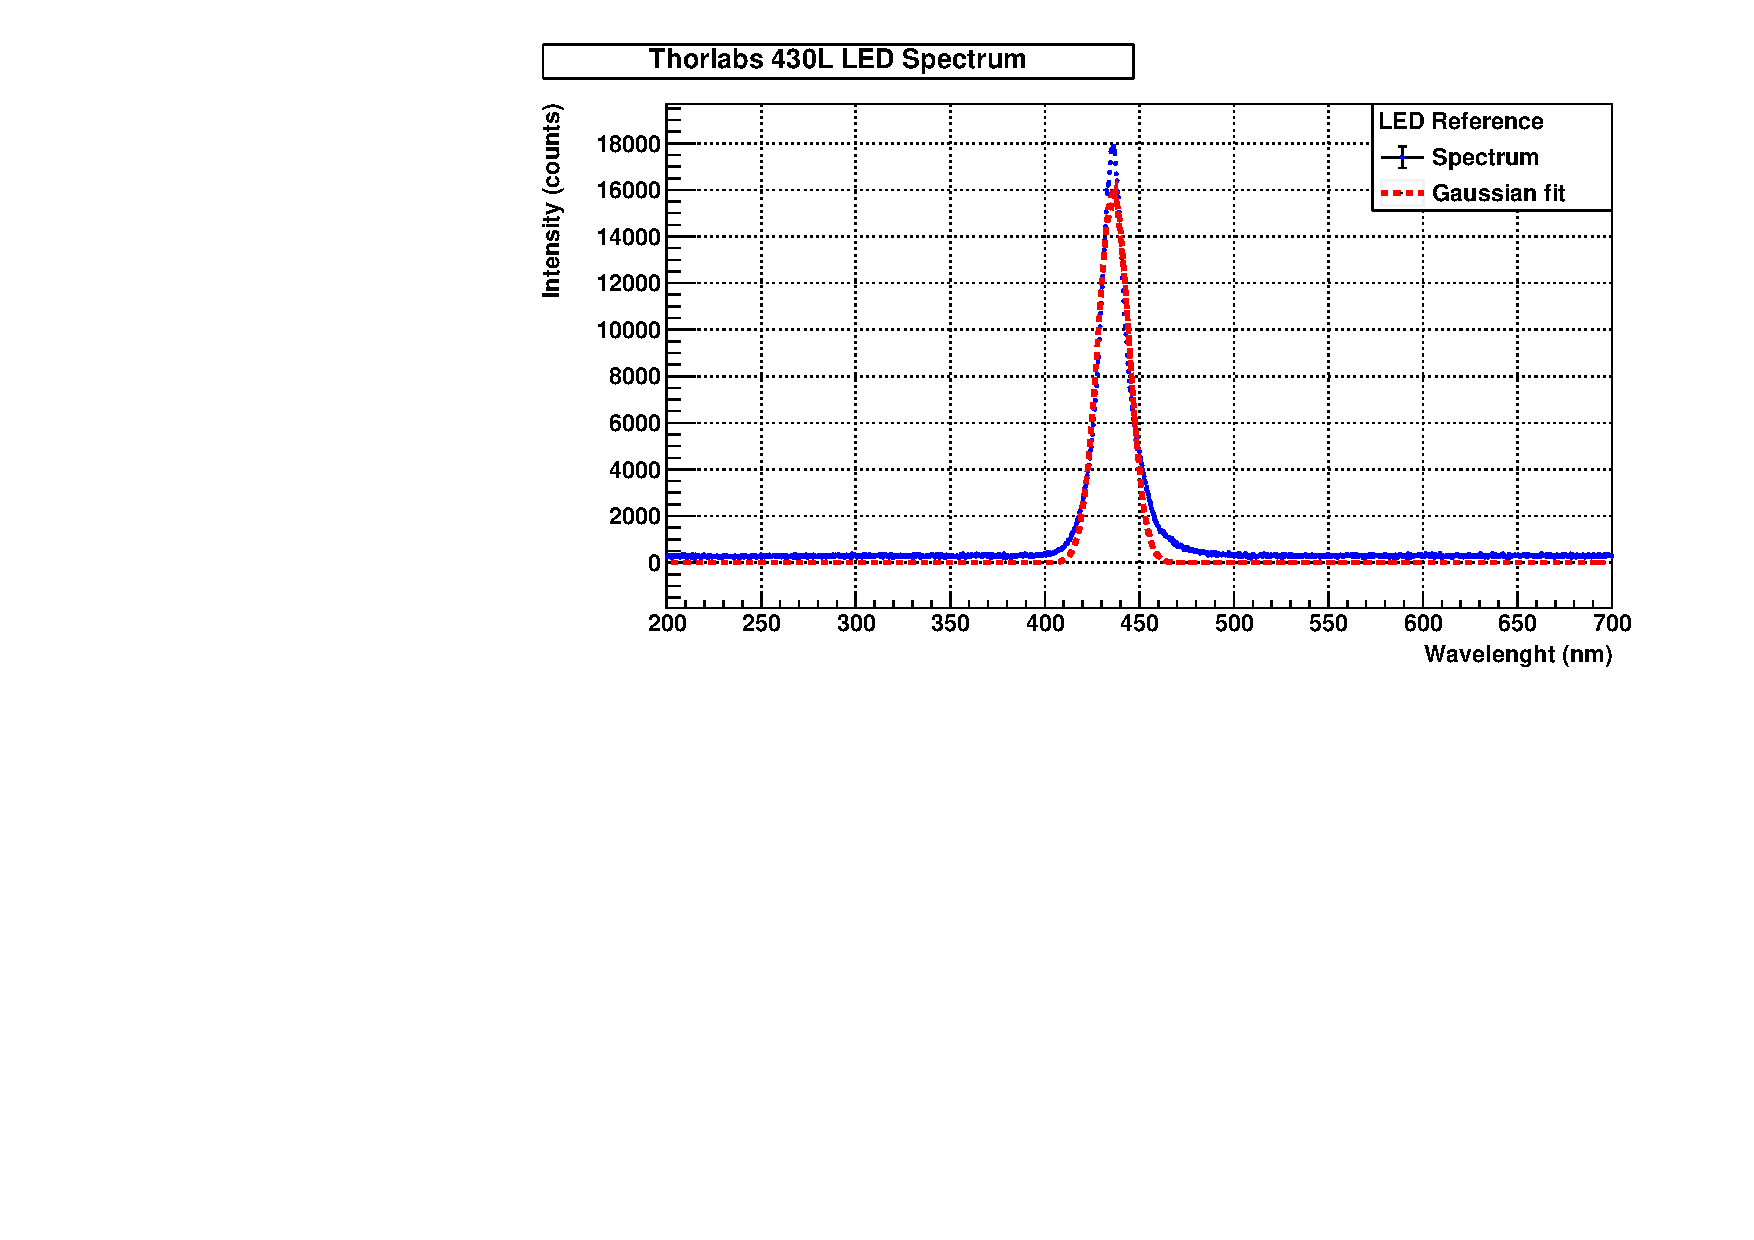
\includegraphics[width=0.6\textwidth]{3DesignPrinciples/32Tritium_detector/LED_DUNE.pdf}}
 \caption{Three PCBs used for the SiPM characterization and LED emission spectrum.}
 \label{fig:PCBs_LEDSpectrum}
\end{figure}

The output signal of the third PCB is connected to an oscilloscope, model ..., where the signal are processed and the data is saved and, subsequently analized by ROOT\footnote{ROOT is a framework for data processing, based on C ++ and object-oriented technology, developed at CERN and widely used in nuclear and particle physics.}.